\chapter{Prototype}
The above outlined key concepts were then developed into the key features of our research prototype, \textit{AmbientTeams}. Before stepping into the core features employed in AmbientTeams and aligning them to the above-mentioned key concepts, a brief introduction into the more technical aspects and a general overview of the application are given.

AmbientTeams is a cross-platform desktop application based on Electron\footnote{\url{https://www.electronjs.org/}}. To facilitate the implementation of the interactive user interface, VueJS\footnote{\url{https://vuejs.org/}} was used. To maintain JavaScript as a common language for the front-end and back-end, NodeJS\footnote{\url{https://nodejs.org/}} is used on the server-side. The server provides both a REST API for basic CRUD functionality for users and teams, as well as a WebSocket endpoint since much of the data required for AmbientTeams comes from the server in real-time.

AmbientTeams comes with two main windows. The team overview window is responsible for maintaining a connection to the server, authenticating, login functionality, settings. Additionally, once the user has authenticated, they are redirected to the team overview view where all teams and team members are visible (see \autoref{fig:at_overview}). By clicking on the edit icon next to the team name, the user can select team members from each team that will then be displayed on the other main window, the ambient window. This is demonstrated in \autoref{fig:at_overview}, where the user is selecting the team members to be displayed on the ambient window.

TODO: Talk about avatar library
TODO: Talk about different team 'types': local and remote


\begin{figure}[h]
    \centering
    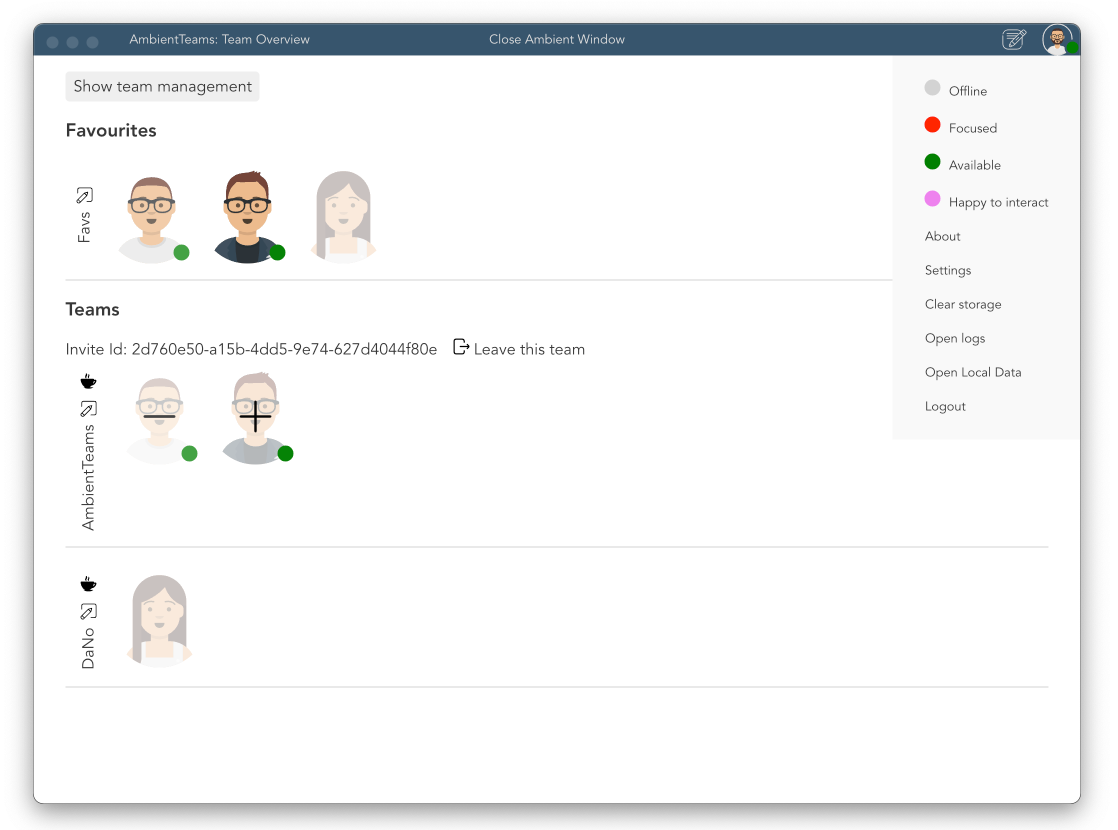
\includegraphics[width=.8\linewidth]{./images/AT_overview.png}
    \caption{Team overview window }
    \label{fig:at_overview}
\end{figure}

\medskip\noindent\textbf{Ambient always-on-top, people-centered team view} \\
AmbientTeams consists of two main windows; a team overview window and the so-called ambient window. The ambient window always sits on top of other windows, making it prone to interruptions and distractions. To keep the ambient overlay as ambient and minimal as possible, we employed a transparent window. Further, certain functionality is only visible when the user is hovering over this window. When hovering over the ambient window, the user can select the team they want to show and sees the names of the individual team members, as shown in \autoref{fig:at_hover}.

\begin{figure}[h]
    \centering
    \begin{subfigure}{.5\textwidth}
        \centering
        
\includegraphics[width=.8\linewidth]{./images/AT_no_hover.png}
        \caption{No hover }
        \label{fig:at_no_hover}
    \end{subfigure}%
    \begin{subfigure}{.5\textwidth}
        \centering
        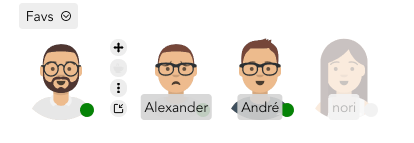
\includegraphics[width=.8\linewidth]{./images/AT_hover.png}
        \caption{Hover }
        \label{fig:at_hover}
    \end{subfigure}
    \caption{Ambient window}
\end{figure}

\medskip\noindent\textbf{Transience and topicality} \\
To ensure that information shared within AmbientTeams is up-to-date, a couple of measures have been taken. The first is a purely visual effect which leads to the avatars fading out when no recent activities took place \autoref{fig:at_no_hover}. Such activities include status and mood sharing, direct messages, and nudging. In addition to potentially motivating users to interact with such faded-out team members, this automatic fading out facilitates spotting colleagues' updates quickly.
Since the goal of AmbientTeams is to foster informal communication, it has no chat history or any other history built into the application. With this transience, we aim to promote less formal communication and hope to avoid the AmbientTeams becomes just another tool to keep track of for work.

TODO: auto-reset status at midnight

\medskip\noindent\textbf{Mood and context sharing} \\
The user can open the sharing window from both the team overview and the ambient window, as well as the system tray menu. All of those actions will open the sharing window as shown in \autoref{fig:sharing_manual}, where on the left, a preview of the current avatar and the selection of predefined moods are listed. There are nine available moods, visualized using popular emoticons. The first four emoticons are more optimistic, the fifth is a neutral face, and the last four are emoticons representing rather negative emotional states. The selection of the emoticons started with the basic emotions surprise, fear, disgust, anger, happiness, or sadness. This list was expanded over time to, in our opinion, suit the work environment better by adding a neutral and tired emoticon, as well as two more positive emotions (loving hearts and grinning) to make the selection more balanced. Due to limitations with the avatar API, we were not able to render the emotion fear well enough, which led us to remove it. On the right, a textbox for providing additional context is shown. The contents of this textbox are, if available, pre-populated with the current status message for the currently selected team. Additionally, the text is highlighted when the window is created, facilitating overwriting the current status without using the mouse to select the text manually. Status messages' length is limited to 140 characters, motivated by the initial limit of Twitter (TODO: cite). Below the textbox, the user can find a button to share the status message with either all teams or a single team.

As a reminder for the user to share his moods and/or additional context with the team members, the sharing window is also automatically scheduled to appear on the lower right corner of the user's primary monitor to minimize the distraction potential. All in all, the window has the same functionality but includes two additional buttons to postpone the prompt for either 5 minutes or 1 hour (see \autoref{fig:sharing_auto}). The scheduled sharing window is shown at three predefined times throughout the day, namely at 9:00, 13:00, and 16:00 local time.

\begin{figure}[h]
    \centering
    \begin{subfigure}{.5\textwidth}
        \centering
        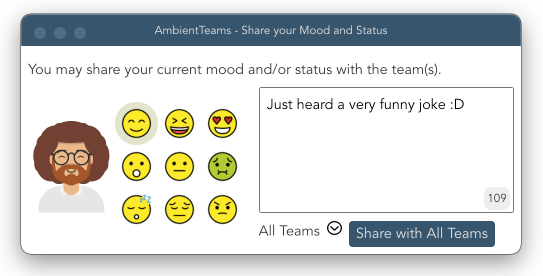
\includegraphics[width=.8\linewidth]{./images/sharing_manual.png}
        \caption{Manually opened }
        \label{fig:sharing_manual}
    \end{subfigure}%
    \begin{subfigure}{.5\textwidth}
        \centering
        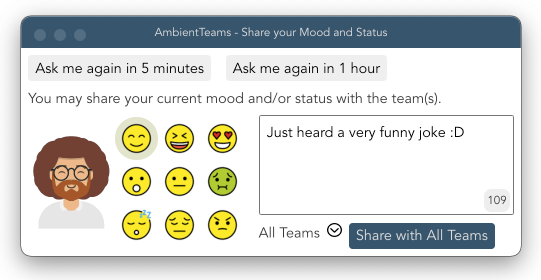
\includegraphics[width=.8\linewidth]{./images/sharing_auto.png}
        \caption{Scheduled }
        \label{fig:sharing_auto}
    \end{subfigure}
    \caption{Sharing window}
\end{figure}

\medskip\noindent\textbf{Ever-running break room} \\
As stated before, our goal was to make the creation of ever-running break rooms as effortless as possible. \autoref{fig:breakroom_initiator} shows the state of the ambient windows when the user clicked on the coffee icon. Having clicked on this coffee icon, the other members of the team see an indication that there is an ongoing break room (see \autoref{fig:breakroom_indicator}). However, to not unnecessarily set up a break room and potentially interrupt the initiating user, the break room is only created once another user clicks on the coffee icon.

\begin{figure}[h]
    \centering
    \begin{subfigure}{.5\textwidth}
        \centering
        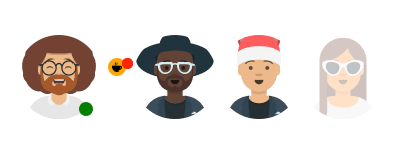
\includegraphics[width=.8\linewidth]{./images/breakroom_initiator.png}
        \caption{Initiating a breakroom creation }
        \label{fig:breakroom_initiator}
    \end{subfigure}%
    \begin{subfigure}{.5\textwidth}
        \centering
        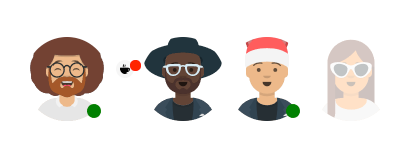
\includegraphics[width=.8\linewidth]{./images/breakroom_indicator.png}
        \caption{Joining a breakroom }
        \label{fig:breakroom_indicator}
    \end{subfigure}
    \caption{Breakroom creation}
\end{figure}


Once at least two team members are interested in a break room, a break room is actually created, and the two are redirected to the break room view (see \autoref{fig:breakroom}). At any point, other team members can join and leave the breakroom, and it stays active as long as at least one team member is part of it. We want to avoid users forgetting the time and staying too long in the break room. For this purpose, whenever a user enters a break room, a 15-minute timer is started. When this timer reaches its end, the user automatically leaves the break room.

\begin{figure}[h]
    \centering
    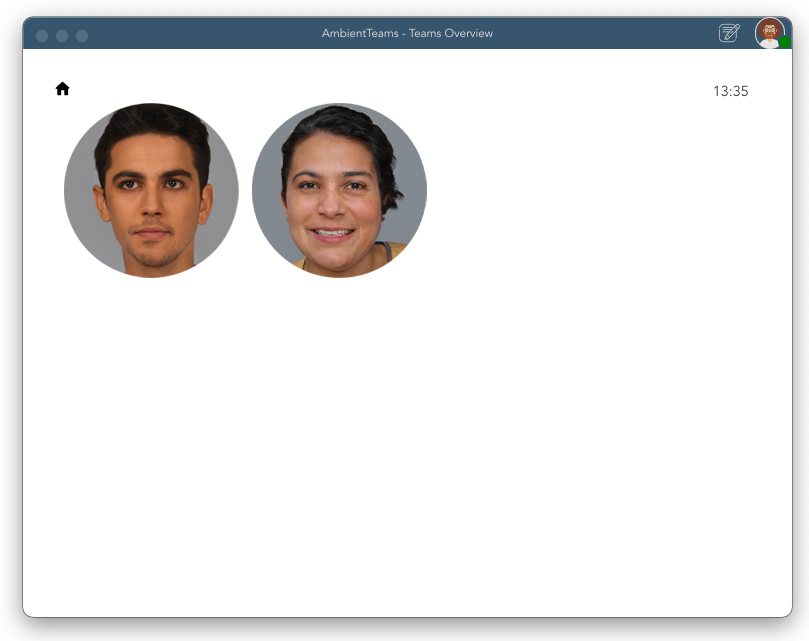
\includegraphics[width=.8\linewidth]{./images/breakroom.png}
    \caption{Breakroom, pictures are artificially created with \url{https://generated.photos/}}
    \label{fig:breakroom}
\end{figure}

\medskip\noindent\textbf{1:1 interactions} \\
Random calls

\medskip\noindent\textbf{Minimizing interruptions} \\
Availibility status -> focus
